% ============================================================================
% arXiv Submission — Scaling Tames Randomness
% Compile: pdflatex main.tex && bibtex main && pdflatex main.tex x2
% ============================================================================
\documentclass[11pt,a4paper]{article}

% ---------- Packages ----------
\usepackage[utf8]{inputenc}
\usepackage[T1]{fontenc}
\usepackage{lmodern}
\usepackage[margin=1in]{geometry}
\usepackage{amsmath,amssymb}
\usepackage{graphicx}
\usepackage{booktabs}
\usepackage{hyperref}
\usepackage{xcolor}
\usepackage{natbib}
\usepackage{caption}
\usepackage{subcaption}
\usepackage{multirow}
\usepackage{array}
\usepackage{float}
\usepackage{enumitem}
\usepackage{microtype}

% ---------- Hyperref setup ----------
\hypersetup{
    colorlinks=true,
    linkcolor=blue!70!black,
    citecolor=green!50!black,
    urlcolor=blue!60!black,
}

% ---------- Custom commands ----------
\newcommand{\ie}{\textit{i.e.}}
\newcommand{\eg}{\textit{e.g.}}
\newcommand{\etal}{\textit{et al.}}
\newcommand{\SI}{\text{SI}}

% ============================================================================
\begin{document}

% ---------- Title ----------
\title{%
    \textbf{Scaling Tames Randomness: A Multi-Metric Investigation of \\
    Output Stochasticity Across Large Language Models \\
    from 0.5\,B to 72\,B Parameters}%
}

\author{
    \textbf{Khashayar Ghamati} \\
    School of Physics, Engineering and Computer Science \\
    University of Hertfordshire \\
    Hatfield AL10 9AB, United Kingdom \\
    \texttt{kg23aay@herts.ac.uk}
}

\date{}

\maketitle

% ============================================================================
% ABSTRACT
% ============================================================================
\begin{abstract}
Large language models (LLMs) generate text through probabilistic sampling, yet the degree to which their outputs vary---and whether that variation changes systematically with model scale---remains poorly quantified.
We present a controlled empirical study that probes the stochasticity of 12 instruction-tuned LLMs spanning three architectural families (Qwen~2.5, LLaMA~3, Gemma~2) and a 144-fold range of parameter counts (0.5\,B to 72\,B).
Each model was prompted 20 times with each of 20 thematically related but distinct questions on AI in healthcare, yielding 4\,800 stateless generations under identical decoding settings (temperature~0.7, top-$p$~0.9).
We evaluate output variability through a battery of 13 complementary metrics drawn from lexical, semantic, and structural analysis, which we aggregate into a single composite \emph{Stochasticity Index}.
Our results reveal a statistically significant negative correlation between parameter count and stochasticity (Spearman $\rho = -0.767$, $p = 0.004$): smaller models produce markedly more diverse---and less predictable---outputs, while larger models converge toward more deterministic response patterns.
A Kruskal--Wallis test confirms that stochasticity differs significantly across four model-size tiers ($H = 137.78$, $p < 10^{-29}$).
We further observe that this relationship is not driven by a single metric but is consistent across 11 of 13 individual measures, suggesting a fundamental shift in generation behaviour as models scale.
These findings carry practical implications for reproducibility, evaluation methodology, and the deployment of LLMs in safety-critical domains.
\end{abstract}

\noindent\textbf{Keywords:} large language models; stochasticity; output variability; model scaling; emergent properties; reproducibility; natural language generation; evaluation metrics

% ============================================================================
% 1. INTRODUCTION
% ============================================================================
\section{Introduction}
\label{sec:introduction}

Every time a large language model is asked the same question, it may give a slightly---or dramatically---different answer.
This fundamental property, known as \emph{stochasticity}, arises from the probabilistic sampling mechanisms that underpin modern text generation.
While some degree of variation is desirable (it prevents outputs from feeling robotic or repetitive), excessive unpredictability poses serious challenges in settings where consistency and reproducibility matter, such as clinical decision support, legal document generation, or automated scientific reasoning.

The past three years have witnessed an extraordinary expansion in LLM scale, with openly available models now ranging from sub-billion to over 70 billion parameters.
Alongside this growth, researchers have documented \emph{emergent capabilities}---qualitative improvements in reasoning, instruction following, and factual accuracy that appear to materialise at certain parameter thresholds~\citep{wei2022emergent,srivastava2022beyond}.
A natural yet largely unexplored question follows: does the stochastic behaviour of LLMs also change as models grow larger?
If a 70-billion-parameter model generates more consistent answers than a 0.5-billion-parameter model under identical sampling conditions, this would have profound implications for how we benchmark, deploy, and trust these systems.

Despite its importance, stochasticity in LLMs has received surprisingly little systematic attention.
Most evaluation benchmarks report a single score per model, implicitly assuming that the answer a model gives on one run is representative of all possible runs.
Reproducibility studies have noted variation across runs~\citep{zheng2023judging}, but few have attempted to \emph{measure} that variation as a dependent variable and correlate it with architectural properties such as parameter count.
Those that have tend to rely on a single metric (\eg, Self-BLEU or response length variance), capturing only one dimension of a multifaceted phenomenon.

In this paper, we address this gap through a carefully controlled experiment designed around four guiding questions:

\begin{enumerate}[leftmargin=2em]
    \item \textbf{How stochastic are modern instruction-tuned LLMs?} We quantify the baseline variability of 12 models across three architectural families.
    \item \textbf{Does parameter count predict stochasticity?} We test the hypothesis that larger models produce more consistent outputs.
    \item \textbf{Is the relationship metric-dependent?} We evaluate whether the scaling effect holds across lexical, semantic, and structural dimensions of variation.
    \item \textbf{Do emergent-property thresholds coincide with stochasticity shifts?} By sampling models at four size tiers aligned with known emergence boundaries, we probe whether transitions in capability correspond to transitions in output consistency.
\end{enumerate}

To answer these questions, we adopt a multi-metric evaluation framework comprising 13 complementary measures---from classical $n$-gram statistics to modern neural approaches such as Semantic Entropy~\citep{kuhn2023semantic} and the Vendi Score~\citep{friedman2023vendi}---aggregated into a single composite Stochasticity Index.
Our experimental design ensures fair comparison: all models receive the same 20 prompts, each repeated 20 times without conversational memory, under identical decoding parameters.
The result is a dataset of 4\,800 model responses that allows both aggregate and fine-grained analysis of output variability.

The remainder of this paper is organised as follows.
Section~\ref{sec:related} reviews related work on LLM evaluation, stochasticity, and emergent properties.
Section~\ref{sec:methods} describes our experimental methodology.
Section~\ref{sec:results} presents the results.
Section~\ref{sec:discussion} discusses implications, limitations, and future directions.
Section~\ref{sec:conclusion} concludes.

% ============================================================================
% 2. RELATED WORK
% ============================================================================
\section{Related Work}
\label{sec:related}

Understanding the variability of LLM outputs requires drawing on several intersecting lines of research: the scaling laws that govern model behaviour, the emergent capabilities that appear at certain scales, and the evaluation methodologies used to quantify text generation quality.

\subsection{Scaling Laws and Emergent Capabilities}

The relationship between model size and performance has been a central theme in LLM research since the seminal work of \citet{kaplan2020scaling}, who demonstrated smooth power-law improvements in loss as a function of parameter count, dataset size, and compute budget.
\citet{hoffmann2022training} refined these laws, showing that many models are undertrained relative to their size and that optimal scaling requires balancing parameters with data volume.

More intriguing than smooth improvements are the \emph{emergent capabilities} documented by \citet{wei2022emergent}: abilities that are absent in smaller models but appear---sometimes abruptly---once a model crosses a size threshold.
Examples include chain-of-thought reasoning, instruction following, and multi-step arithmetic.
\citet{schaeffer2023emergent} later argued that some apparent emergences are artefacts of metric choice, but the consensus remains that qualitative shifts in model behaviour do accompany scale increases, particularly in the 3\,B to 13\,B parameter range for instruction-tuned models.

What has not been studied, however, is whether \emph{output consistency}---the degree to which a model gives similar answers to the same question across runs---also changes with scale.
Our work fills this gap by treating stochasticity itself as the dependent variable in a scaling analysis.

\subsection{Measuring Text Diversity and Consistency}

The NLP community has developed a rich toolkit for measuring how diverse or repetitive a set of generated texts is.
Self-BLEU~\citep{zhu2018texygen} adapts the classic BLEU metric to measure intra-set similarity: each text is scored against all others as references, with high Self-BLEU indicating low diversity.
ROUGE-L~\citep{lin2004rouge} captures longest-common-subsequence overlap and is widely used for summarisation evaluation.
TF-IDF cosine similarity~\citep{salton1988term} provides a term-frequency-weighted perspective on lexical overlap.

At the semantic level, embedding-based cosine similarity uses dense vector representations to capture meaning beyond surface forms.
More recently, \citet{kuhn2023semantic} introduced \emph{Semantic Entropy}, which clusters responses by meaning and computes Shannon entropy over the cluster distribution.
\citet{friedman2023vendi} proposed the \emph{Vendi Score}, an eigenvalue-based diversity metric derived from the kernel similarity matrix, which elegantly captures the effective number of distinct outputs.

Most of these metrics have been applied in isolation.
Our contribution is to deploy them as a \emph{battery} and examine whether their signals converge---testing whether the scaling effect on stochasticity is a robust phenomenon or an artefact of a particular measurement approach.

\subsection{Reproducibility in LLM Evaluation}

The reproducibility crisis in machine learning~\citep{pineau2021improving} is particularly acute for LLMs, where a single evaluation run may not reflect a model's typical behaviour.
\citet{zheng2023judging} showed that LLM-as-a-judge scores vary across runs, and \citet{biderman2023pythia} demonstrated that benchmark rankings can change depending on the random seed.
These observations motivate our experimental design: by repeating each prompt 20 times, we can characterise the \emph{distribution} of outputs, not just a point estimate, and quantify how that distribution changes with model scale.

% ============================================================================
% 3. MATERIALS AND METHODS
% ============================================================================
\section{Materials and Methods}
\label{sec:methods}

Designing a fair comparison of stochasticity across models of vastly different sizes requires careful attention to experimental controls.
In this section, we describe how we selected models, designed prompts, configured generation parameters, and defined our evaluation metrics, with the goal of isolating the effect of parameter count while minimising confounding factors.

\subsection{Model Selection}
\label{sec:models}

We selected 12 instruction-tuned LLMs from three architectural families, spanning a 144-fold range of parameter counts from 0.5 billion to 72 billion.
Table~\ref{tab:models} summarises the models and their tier assignments.

\begin{table}[t]
\centering
\caption{Models evaluated, organised by tier. All models are instruction-tuned variants accessed via HuggingFace Transformers.}
\label{tab:models}
\small
\begin{tabular}{@{}clllr@{}}
\toprule
\textbf{Tier} & \textbf{Label} & \textbf{Model} & \textbf{Family} & \textbf{Params} \\
\midrule
\multirow{4}{*}{1} & \multirow{4}{*}{Small}
  & Qwen/Qwen2.5-0.5B-Instruct       & Qwen 2.5 & 0.5\,B \\
& & meta-llama/Llama-3.2-1B-Instruct  & LLaMA 3  & 1.0\,B \\
& & Qwen/Qwen2.5-1.5B-Instruct       & Qwen 2.5 & 1.5\,B \\
& & google/gemma-2-2b-it              & Gemma 2  & 2.0\,B \\
\midrule
\multirow{4}{*}{2} & \multirow{4}{*}{Medium}
  & Qwen/Qwen2.5-3B-Instruct         & Qwen 2.5 & 3.0\,B \\
& & meta-llama/Llama-3.2-3B-Instruct  & LLaMA 3  & 3.0\,B \\
& & Qwen/Qwen2.5-7B-Instruct         & Qwen 2.5 & 7.0\,B \\
& & meta-llama/Llama-3.1-8B-Instruct  & LLaMA 3  & 8.0\,B \\
\midrule
\multirow{2}{*}{3} & \multirow{2}{*}{Large}
  & google/gemma-2-9b-it              & Gemma 2  & 9.0\,B \\
& & Qwen/Qwen2.5-14B-Instruct        & Qwen 2.5 & 14.0\,B \\
\midrule
\multirow{2}{*}{4} & \multirow{2}{*}{Frontier}
  & meta-llama/Llama-3.1-70B-Instruct & LLaMA 3  & 70.0\,B \\
& & Qwen/Qwen2.5-72B-Instruct        & Qwen 2.5 & 72.0\,B \\
\bottomrule
\end{tabular}
\end{table}

The tier boundaries were chosen to align with documented emergent-capability thresholds.
Tier~1 (below 3\,B) represents models that typically lack robust instruction-following abilities.
Tier~2 (3--8\,B) captures the range where instruction following and basic reasoning begin to emerge.
Tier~3 (9--32\,B) corresponds to models exhibiting more consistent reasoning and factual accuracy.
Tier~4 (70\,B and above) represents frontier models with full emergent capabilities.

We deliberately included multiple families at overlapping sizes (\eg, Qwen~3\,B and LLaMA~3.2~3\,B are both 3\,B but from different architectures) to distinguish scale effects from family-specific effects.

\subsection{Prompt Design}
\label{sec:prompts}

To ensure a controlled yet realistic evaluation, we designed 20 prompts centred on a single domain---\emph{Artificial Intelligence in Healthcare}---but each approaching the topic from a distinct angle.
The 20 angles span the breadth of the domain: general overview, medical diagnostics, drug discovery, patient data privacy, rural healthcare access, mental health, cost reduction, robotic surgery, personalised medicine, electronic health records, clinical trials, ethics, medical imaging, elderly care, pandemic response, medical education, billing and insurance, rare diseases, preventive care, and regulatory challenges.

Anchoring all prompts to a single domain serves two purposes.
First, it ensures that all models are evaluated on comparable content, eliminating domain difficulty as a confound.
Second, it allows us to probe whether certain sub-topics elicit more stochastic behaviour than others---a nuance that would be lost in a multi-domain design.

Each prompt concludes with an identical structured output template requiring the model to return a JSON object with six fields: a two-to-three sentence summary, five key points, three challenges, a potential impact statement, a confidence level (high, medium, or low), and an estimated timeline (short-term, medium-term, or long-term).
This structured format serves a dual role: it standardises outputs for fair comparison and enables \emph{structural} metrics (\eg, template adherence, key-point consistency) alongside lexical and semantic ones.

\subsection{Experimental Protocol}
\label{sec:protocol}

Each of the 20 prompts was sent to each model 20 times independently, yielding 400 generations per model and 4\,800 in total across all 12 models.
Critically, each generation was \emph{stateless}: no conversational history was carried between repetitions, and no system prompt was varied.
This ensures that any observed variation arises solely from the sampling process, not from contextual differences.

All models were served through HuggingFace Transformers with identical decoding parameters:
\begin{itemize}[leftmargin=2em,itemsep=2pt]
    \item \textbf{Temperature:} 0.7 (moderate stochasticity)
    \item \textbf{Top-$p$ (nucleus sampling):} 0.9
    \item \textbf{Maximum tokens:} 1\,024
    \item \textbf{Random seed:} None (non-deterministic)
\end{itemize}

Models with fewer than 27\,B parameters were loaded in FP16 precision.
Models between 27\,B and 65\,B were quantised to 8-bit, and models above 65\,B to 4-bit, using the BitsAndBytes library~\citep{dettmers2023qlora}.
All experiments were executed on a SLURM-managed GPU cluster equipped with NVIDIA A100 80\,GB GPUs at the University of Hertfordshire.

\subsection{Evaluation Metrics}
\label{sec:metrics}

We assessed output stochasticity through 13 metrics spanning three categories: lexical, semantic, and structural.
This multi-dimensional approach is motivated by the recognition that two sets of outputs can be lexically diverse yet semantically identical (paraphrasing) or lexically similar yet structurally inconsistent.

\subsubsection{Lexical Metrics}

\textbf{Self-BLEU}~\citep{zhu2018texygen}.
For each response in a set of 20, we compute BLEU-4 against all other responses as references, then average.
High Self-BLEU indicates high inter-response similarity (low stochasticity).

\textbf{ROUGE-L (Pairwise)}~\citep{lin2004rouge}.
We compute the ROUGE-L F1 score for every pair of responses and average.
ROUGE-L captures the longest common subsequence, making it sensitive to structural word-order similarity.

\textbf{Jaccard Similarity (Pairwise).}
For each pair of responses, we compute the ratio of shared tokens to total unique tokens.
This bag-of-words measure complements BLEU and ROUGE by ignoring word order.

\textbf{TF-IDF Cosine Similarity (Pairwise)}~\citep{salton1988term}.
We vectorise responses using term frequency--inverse document frequency and compute pairwise cosine similarities.
TF-IDF downweights common words, emphasising content-bearing term overlap.

\textbf{Unique $N$-gram Ratio.}
We pool all trigrams from the 20 responses and compute the fraction that are unique.
High uniqueness indicates high lexical diversity.

\subsubsection{Semantic Metrics}

\textbf{Embedding Cosine Similarity.}
We embed each response using the all-MiniLM-L6-v2 sentence transformer~\citep{reimers2019sentence} and compute pairwise cosine similarities.
Unlike lexical metrics, embedding similarity captures whether responses \emph{mean} the same thing, even if they use different words.

\textbf{Semantic Entropy}~\citep{kuhn2023semantic}.
Following Kuhn~\etal, we cluster response embeddings using agglomerative clustering with a cosine-distance threshold of 0.15, then compute normalised Shannon entropy over the cluster distribution.
High entropy means the model produces semantically distinct answers; zero entropy means all responses fall into a single meaning cluster.

\textbf{Vendi Score}~\citep{friedman2023vendi}.
We construct the normalised cosine-similarity kernel matrix over the response embeddings and compute the exponential of the Shannon entropy of its eigenvalues.
The Vendi Score approximates the effective number of distinct responses and is normalised to $[0, 1]$ by dividing by~$n$.

\subsubsection{Structural Metrics}

\textbf{Template Adherence Rate.}
The fraction of responses that parse as valid JSON and contain all six expected fields.

\textbf{Response Length CV.}
The coefficient of variation (standard deviation divided by mean) of response character counts.

\textbf{Key-Point Consistency.}
For responses that successfully parse as JSON, we extract the five key points, tokenise them into word bags, and compute pairwise Jaccard similarity.

\textbf{Confidence-Level Consistency.}
The frequency of the modal confidence-level value across the 20~responses.

\textbf{Timeline Consistency.}
Analogous to confidence consistency, but for the estimated-timeline field.

\subsubsection{Composite Stochasticity Index}

To synthesise the 13 individual metrics into a single score, we define a weighted Stochasticity Index~(SI).
Similarity-oriented metrics are inverted ($1 - \text{value}$) so that high values indicate high stochasticity; diversity-oriented metrics are used directly.
All values are clipped to $[0, 1]$ and combined via a weighted average:
\begin{equation}
\label{eq:si}
\text{SI} = \frac{\sum_{i} w_i \cdot s_i}{\sum_{i} w_i}
\end{equation}
where $s_i$ is the (possibly inverted) metric value and $w_i$ is its weight.
The weights reflect the relative informativeness of each metric category: semantic metrics receive the highest weights (Semantic Entropy: 0.15, Embedding Cosine: 0.12, Vendi Score: 0.10), lexical metrics receive moderate weights (0.05--0.10), and structural metrics receive lower weights (0.04--0.06).
The resulting SI ranges from 0 (perfectly deterministic) to 1 (maximally stochastic).

\subsection{Statistical Analysis}
\label{sec:stats}

We employ the following statistical tests:
\begin{itemize}[leftmargin=2em,itemsep=2pt]
    \item \textbf{Spearman rank correlation} between parameter count and SI, chosen because the relationship need not be linear and parameter counts are highly skewed.
    \item \textbf{Pearson correlation} for comparison, testing the linear association.
    \item \textbf{Kruskal--Wallis $H$-test} across the four model-size tiers, using per-prompt SI values (240 observations) to test whether at least one tier differs significantly.
    \item \textbf{Per-metric Spearman correlations} to identify which individual metrics drive the aggregate trend.
\end{itemize}
All $p$-values are reported at the $\alpha = 0.05$ significance level.

% ============================================================================
% 4. RESULTS
% ============================================================================
\section{Results}
\label{sec:results}

We now present our findings, moving from the broadest view---the overall relationship between model size and stochasticity---to progressively finer-grained analyses of individual metrics, model families, and prompt angles.

\subsection{Aggregate Stochasticity Across Model Scales}
\label{sec:aggregate}

Figure~\ref{fig:scatter} plots each model's aggregate Stochasticity Index against its parameter count, revealing a clear downward trend: smaller models are substantially more stochastic than larger ones.

\begin{figure}[t]
\centering
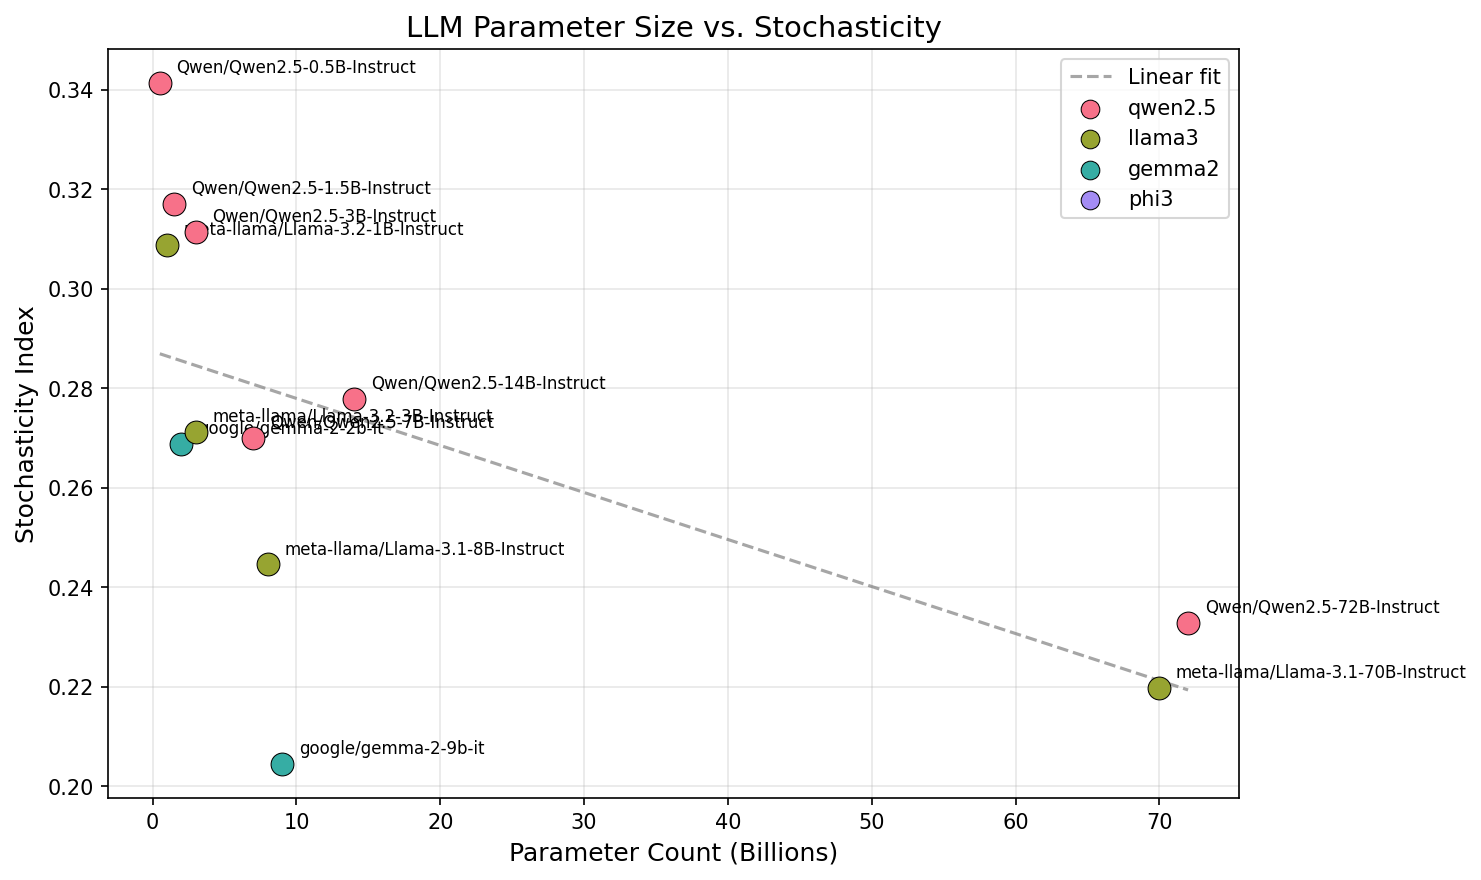
\includegraphics[width=\linewidth]{figures/params_vs_stochasticity.png}
\caption{Parameter count vs.\ Stochasticity Index for all 12 models. The dashed line shows the linear fit. Colour encodes model family. The downward trend is statistically significant (Spearman $\rho = -0.767$, $p = 0.004$).}
\label{fig:scatter}
\end{figure}

Table~\ref{tab:ranking} presents the full ranking.
The most stochastic model, Qwen2.5-0.5B (SI~$= 0.341$), scores 67\% higher than the least stochastic, Gemma-2-9b (SI~$= 0.205$).

\begin{table}[t]
\centering
\caption{Stochasticity Index by model, sorted from most to least stochastic. Values report the mean $\pm$ standard deviation across 20 prompts.}
\label{tab:ranking}
\small
\begin{tabular}{@{}clcrc@{}}
\toprule
\textbf{Rank} & \textbf{Model} & \textbf{Family} & \textbf{Params} & \textbf{SI (mean $\pm$ std)} \\
\midrule
1  & Qwen2.5-0.5B   & Qwen 2.5 &  0.5\,B & $0.341 \pm 0.021$ \\
2  & Qwen2.5-1.5B   & Qwen 2.5 &  1.5\,B & $0.317 \pm 0.019$ \\
3  & Qwen2.5-3B     & Qwen 2.5 &  3.0\,B & $0.312 \pm 0.015$ \\
4  & Llama-3.2-1B   & LLaMA 3  &  1.0\,B & $0.309 \pm 0.025$ \\
5  & Qwen2.5-14B    & Qwen 2.5 & 14.0\,B & $0.278 \pm 0.027$ \\
6  & Llama-3.2-3B   & LLaMA 3  &  3.0\,B & $0.271 \pm 0.021$ \\
7  & Qwen2.5-7B     & Qwen 2.5 &  7.0\,B & $0.270 \pm 0.017$ \\
8  & Gemma-2-2b     & Gemma 2  &  2.0\,B & $0.269 \pm 0.011$ \\
9  & Llama-3.1-8B   & LLaMA 3  &  8.0\,B & $0.245 \pm 0.023$ \\
10 & Qwen2.5-72B    & Qwen 2.5 & 72.0\,B & $0.233 \pm 0.017$ \\
11 & Llama-3.1-70B  & LLaMA 3  & 70.0\,B & $0.220 \pm 0.013$ \\
12 & Gemma-2-9b     & Gemma 2  &  9.0\,B & $0.205 \pm 0.014$ \\
\bottomrule
\end{tabular}
\end{table}

The Spearman rank correlation between parameter count and Stochasticity Index is $\rho = -0.767$ ($p = 0.004$), indicating a strong and statistically significant negative monotonic relationship.
The Pearson correlation is $r = -0.587$ ($p = 0.045$), also significant, though weaker owing to the non-linear distribution of parameter counts.

\subsection{Tier-Level Analysis}
\label{sec:tiers}

To test whether stochasticity differs across model-size groups aligned with emergent-capability thresholds, we conducted a Kruskal--Wallis test using per-prompt SI values grouped into four tiers.
The result is highly significant: $H = 137.78$, $p < 10^{-29}$.

This confirms that the trend is not merely a smooth gradient; there are statistically meaningful \emph{jumps} in output consistency between model-size categories.
The median SI decreases monotonically from Tier~1 (small, $\approx\!0.33$) through Tier~2 (medium, $\approx\!0.28$) and Tier~3 (large, $\approx\!0.24$) to Tier~4 (frontier, $\approx\!0.23$).
The largest drop occurs between Tiers~1 and~2, suggesting that the transition from sub-3\,B to 3--8\,B models represents the most impactful scaling step for output consistency.

\begin{figure}[t]
\centering
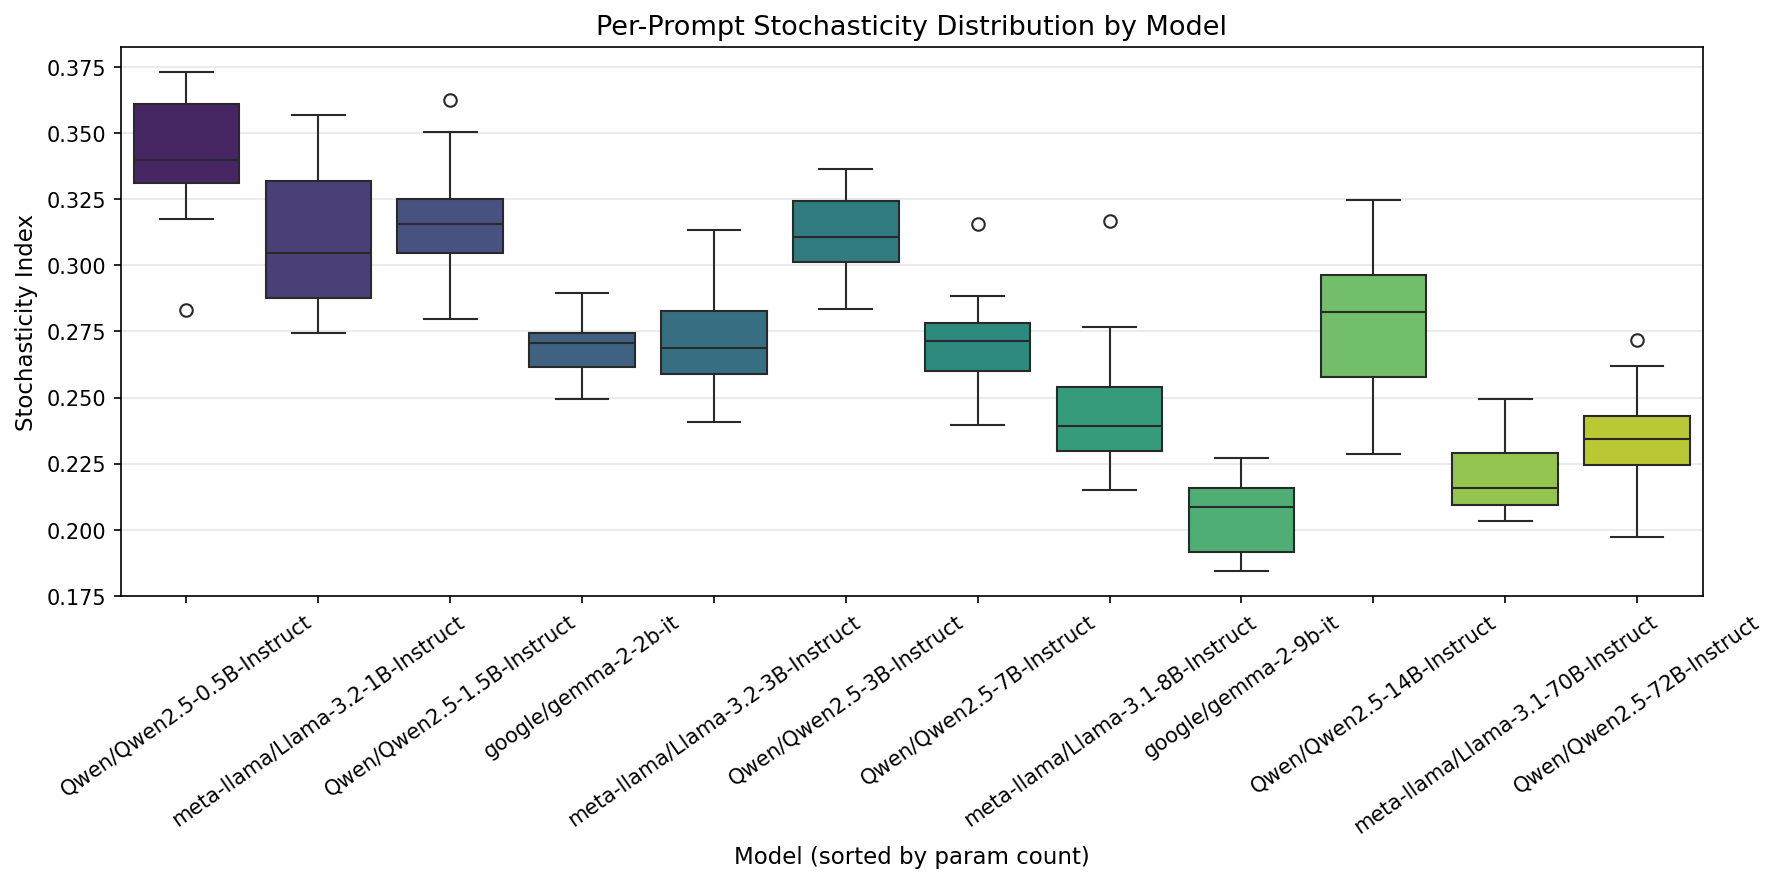
\includegraphics[width=\linewidth]{figures/stochasticity_boxplot.png}
\caption{Per-prompt Stochasticity Index distribution by model, sorted by parameter count (left to right). Boxes show the interquartile range; whiskers extend to 1.5$\times$\,IQR. The systematic decrease with model size is clearly visible.}
\label{fig:boxplot}
\end{figure}

\subsection{Per-Metric Correlations: A Consistent Signal}
\label{sec:permetric}

A natural concern is that the composite Stochasticity Index might be dominated by one or two metrics.
Table~\ref{tab:correlations} addresses this by reporting the Spearman correlation of each individual metric with parameter count.

\begin{table}[t]
\centering
\caption{Per-metric Spearman correlations with parameter count. Asterisks denote significance at $p < 0.05$.}
\label{tab:correlations}
\small
\begin{tabular}{@{}llcrl@{}}
\toprule
\textbf{Metric} & \textbf{Category} & \textbf{$\rho$} & \textbf{$p$} & \textbf{Interpretation} \\
\midrule
Self-BLEU            & Lexical    & $+0.771$* & 0.003 & More self-similar \\
ROUGE-L              & Lexical    & $+0.676$* & 0.016 & More overlapping \\
Jaccard              & Lexical    & $+0.708$* & 0.010 & More shared tokens \\
TF-IDF Cosine        & Lexical    & $+0.522$  & 0.082 & Trend, not significant \\
Unique $N$-gram \%   & Lexical    & $-0.701$* & 0.011 & Fewer unique $n$-grams \\
\midrule
Embedding Cosine     & Semantic   & $+0.644$* & 0.024 & Semantically closer \\
Semantic Entropy     & Semantic   & $-0.618$* & 0.032 & Lower entropy \\
Vendi Score          & Semantic   & $-0.644$* & 0.024 & Less diverse \\
\midrule
Template Adherence   & Structural & $+0.650$* & 0.022 & Better format following \\
Length CV            & Structural & $-0.781$* & 0.003 & More consistent length \\
Key-Point Consist.   & Structural & $+0.658$* & 0.020 & More consistent content \\
Confidence Consist.  & Structural & $+0.032$  & 0.923 & No relationship \\
Timeline Consist.    & Structural & $+0.806$* & 0.002 & More consistent timeline \\
\bottomrule
\end{tabular}
\end{table}

The results are striking: 11 of 13 metrics show a significant correlation with parameter count, and all in the direction that larger models are less stochastic.
The two exceptions are TF-IDF cosine similarity (trending but not significant, $p = 0.082$) and confidence-level consistency (effectively flat, $\rho = 0.032$, $p = 0.923$).

The consistency across metric categories is particularly compelling.
Whether we measure variation through lexical overlap (Self-BLEU, $\rho = +0.771$), semantic clustering (Semantic Entropy, $\rho = -0.618$), or structural reliability (Length CV, $\rho = -0.781$), the conclusion is the same: larger models produce more consistent outputs.

The lone holdout---confidence-level consistency---is readily explained.
Most models, regardless of size, assign ``medium'' confidence to healthcare AI topics, yielding near-ceiling consistency scores (mean 0.915) with almost no variance to correlate.

\subsection{Metric Profiles: A Deeper Look}
\label{sec:profiles}

\begin{figure}[t]
\centering
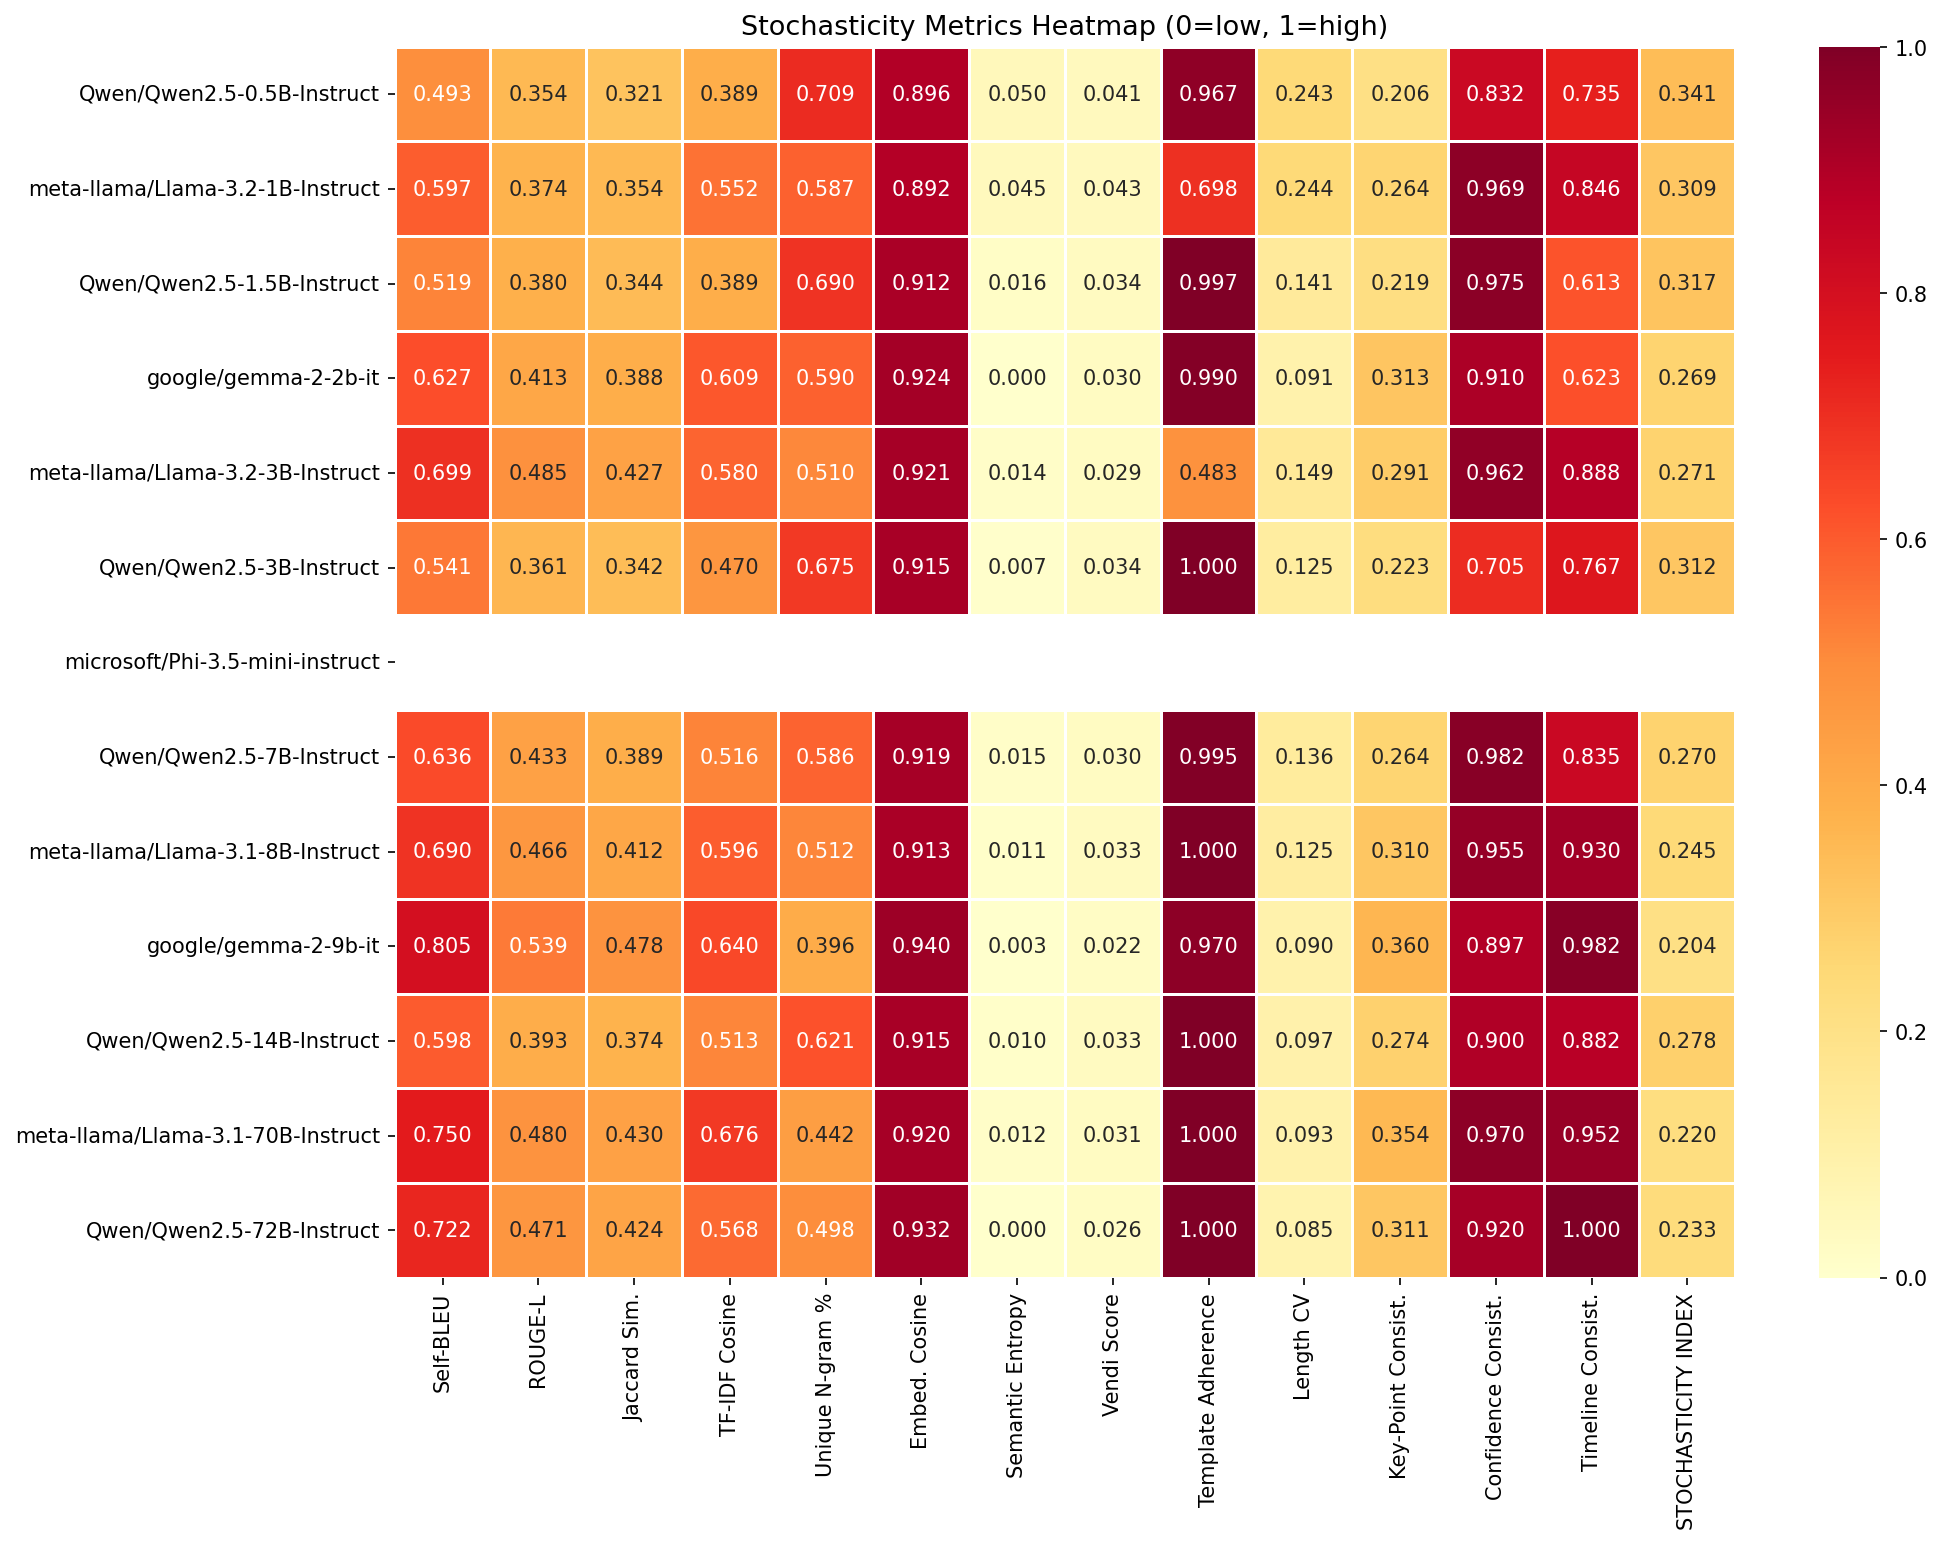
\includegraphics[width=\linewidth]{figures/metrics_heatmap.png}
\caption{Heatmap of all 13 metric values (columns) for each model (rows), sorted by parameter count. The Phi-3.5 row is blank due to data collection failure. Warmer colours indicate higher values.}
\label{fig:heatmap}
\end{figure}

Beyond correlations, the absolute metric values reveal the \emph{character} of stochasticity at different scales (Table~\ref{tab:descriptive}).

\begin{table}[t]
\centering
\caption{Descriptive statistics of evaluation metrics across all 12 models.}
\label{tab:descriptive}
\small
\begin{tabular}{@{}lcccc@{}}
\toprule
\textbf{Metric} & \textbf{Mean} & \textbf{Std} & \textbf{Min} & \textbf{Max} \\
\midrule
Self-BLEU             & 0.640 & 0.096 & 0.493 & 0.805 \\
ROUGE-L               & 0.429 & 0.059 & 0.354 & 0.539 \\
Jaccard Similarity    & 0.390 & 0.046 & 0.321 & 0.478 \\
TF-IDF Cosine         & 0.542 & 0.091 & 0.389 & 0.676 \\
Unique $N$-gram Ratio & 0.568 & 0.099 & 0.396 & 0.709 \\
\midrule
Embedding Cosine      & 0.916 & 0.013 & 0.892 & 0.941 \\
Semantic Entropy      & 0.015 & 0.016 & 0.000 & 0.050 \\
Vendi Score           & 0.032 & 0.006 & 0.022 & 0.043 \\
\midrule
Template Adherence    & 0.925 & 0.164 & 0.483 & 1.000 \\
Length CV             & 0.135 & 0.055 & 0.086 & 0.244 \\
Key-Point Consist.    & 0.282 & 0.050 & 0.206 & 0.360 \\
Confidence Consist.   & 0.915 & 0.080 & 0.705 & 0.983 \\
Timeline Consist.     & 0.838 & 0.130 & 0.613 & 1.000 \\
\bottomrule
\end{tabular}
\end{table}

Several patterns merit attention.
First, embedding cosine similarity is uniformly high (mean 0.916, range 0.892--0.941), indicating that even the most stochastic models rarely produce \emph{semantically contradictory} answers---the variation is primarily in \emph{phrasing} and \emph{emphasis}, not in \emph{meaning}.
Second, semantic entropy is near zero for most models (mean 0.015), confirming that responses almost always cluster into a single semantic group.

Third, template adherence varies dramatically at the small end.
The 3\,B LLaMA model achieves only 48.3\% template adherence, while most models above 7\,B achieve 99--100\%.
This aligns with the emergent-capability literature: reliably following a structured output format is itself an ability that scales with model size.

\subsection{Family-Level Analysis}
\label{sec:families}

Including three architectural families allows us to separate scaling effects from family-specific effects.
Figure~\ref{fig:family} shows that within each family, stochasticity consistently decreases with size:

\begin{itemize}[leftmargin=2em,itemsep=2pt]
    \item \textbf{Qwen 2.5:} SI drops from 0.341 (0.5\,B) to 0.233 (72\,B)---a 32\% reduction.
    \item \textbf{LLaMA 3:} SI drops from 0.309 (1\,B) to 0.220 (70\,B)---a 29\% reduction.
    \item \textbf{Gemma 2:} SI drops from 0.269 (2\,B) to 0.205 (9\,B)---a 24\% reduction.
\end{itemize}

\begin{figure}[t]
\centering
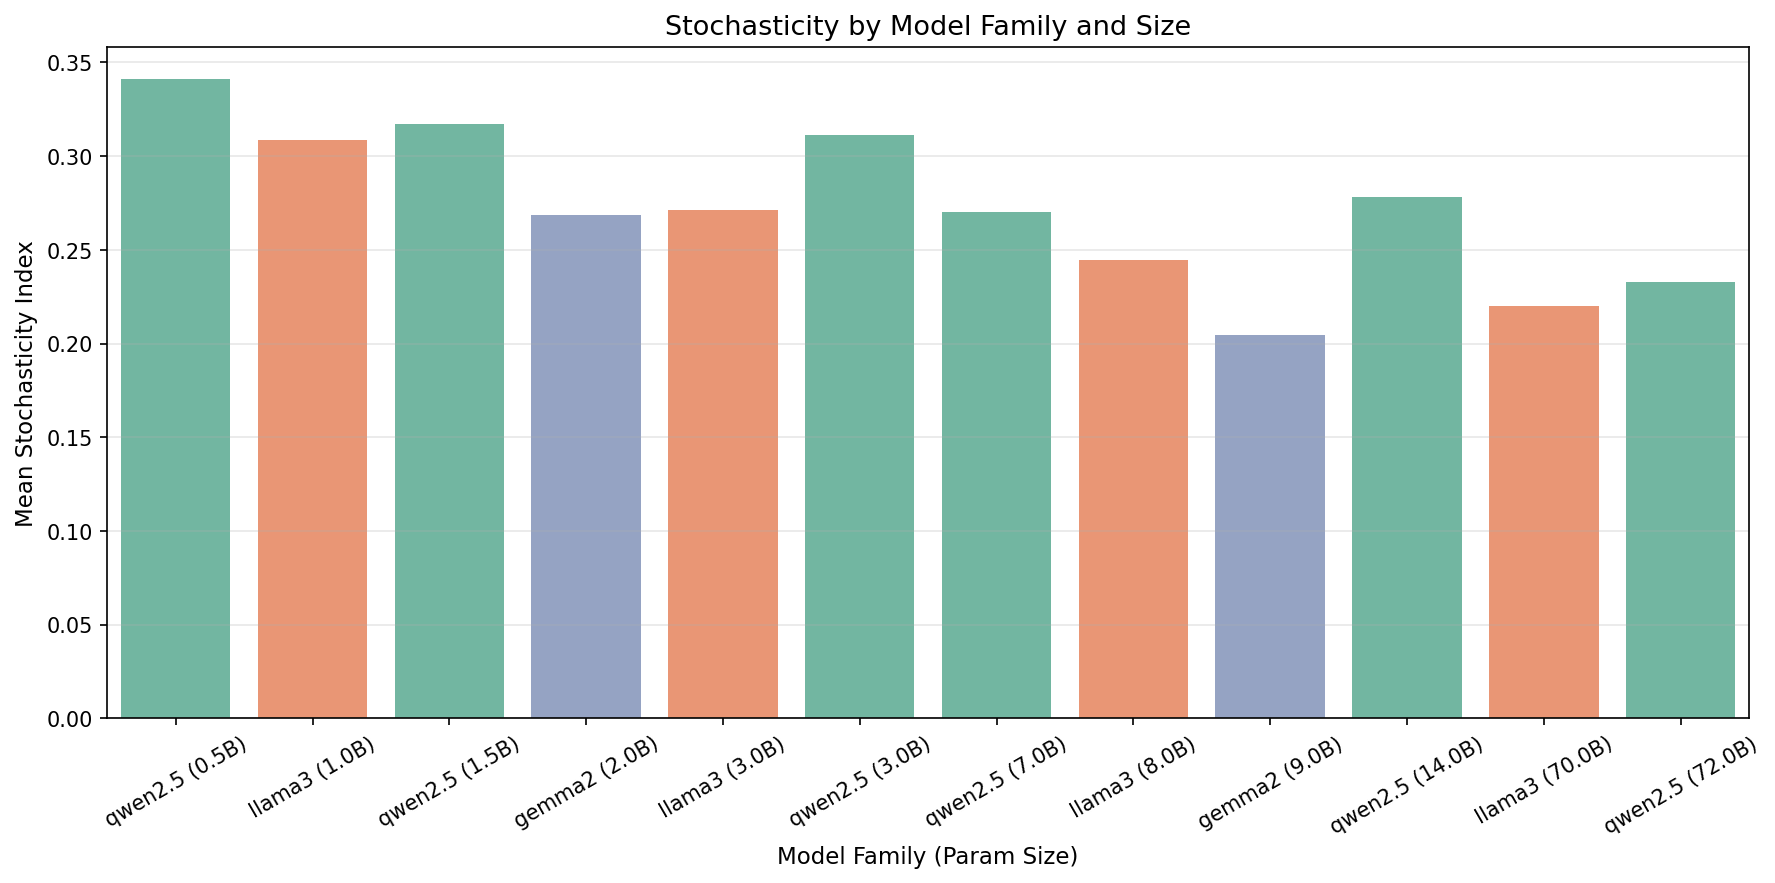
\includegraphics[width=\linewidth]{figures/family_comparison.png}
\caption{Mean Stochasticity Index by model family and parameter count. Within every family, stochasticity decreases with scale.}
\label{fig:family}
\end{figure}

The cross-family consistency reinforces our conclusion that the scaling--stochasticity relationship is a general property of language models, not an artefact of one particular architecture.

Interestingly, at matched parameter counts, the families differ.
At 3\,B, Qwen~2.5 (SI~$= 0.312$) is notably more stochastic than LLaMA~3 (SI~$= 0.271$).
This suggests that training data, alignment procedure, and architectural details all modulate stochasticity independently of scale.

\subsection{Prompt-Level Analysis: Does Topic Angle Matter?}
\label{sec:prompts_analysis}

Figure~\ref{fig:prompt_heatmap} reveals that stochasticity varies not only across models but also across prompt topics, though the model-size effect dominates.

\begin{figure}[t]
\centering
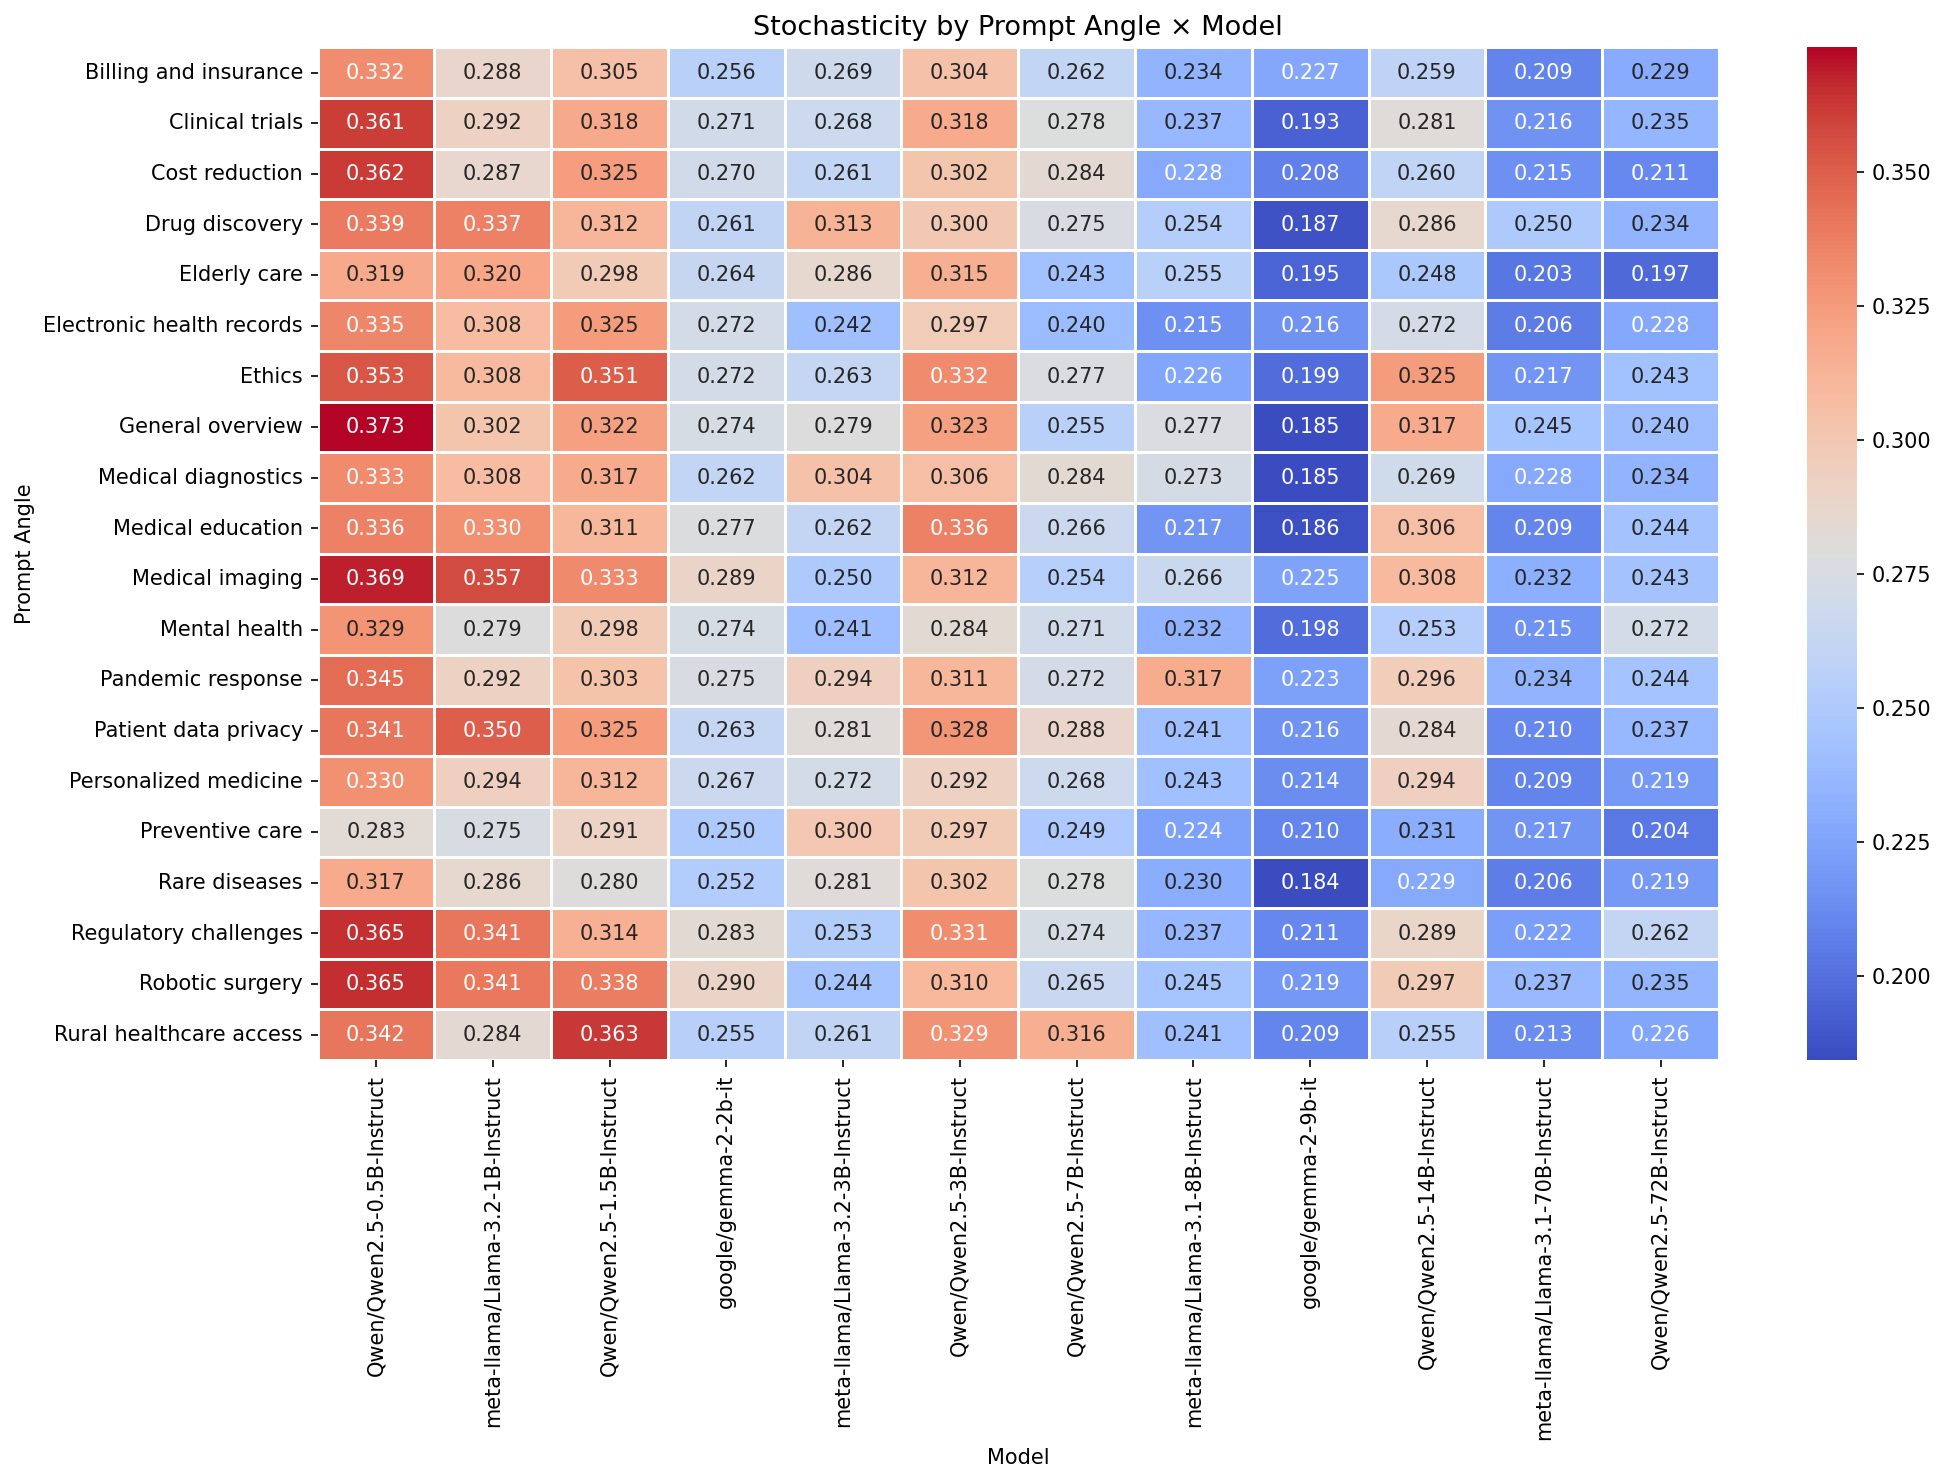
\includegraphics[width=\linewidth]{figures/prompt_angle_heatmap.png}
\caption{Stochasticity Index per prompt angle (rows) and model (columns, sorted by parameter count). Blue indicates low stochasticity; red indicates high. The left-to-right gradient (small$\to$large models) dominates, but row-level variation reveals topic effects.}
\label{fig:prompt_heatmap}
\end{figure}

\textbf{High-stochasticity prompts} (consistently red across models): ``General overview,'' ``Ethics,'' ``Robotic surgery,'' and ``Regulatory challenges.''
These are topics with broad scope and multiple valid framings, inviting diverse responses.
\textbf{Low-stochasticity prompts} (consistently blue): ``Preventive care'' and ``Elderly care.''
These are more concrete, narrower topics where models converge on similar content.

The interaction between prompt angle and model size is also informative.
Small models show high variability across \emph{all} topics, while large models show lower variability overall but with greater \emph{relative} sensitivity to topic difficulty.
This suggests that as models scale, they develop more nuanced topic sensitivity while simultaneously becoming more consistent in their baseline behaviour.

\begin{figure}[t]
\centering
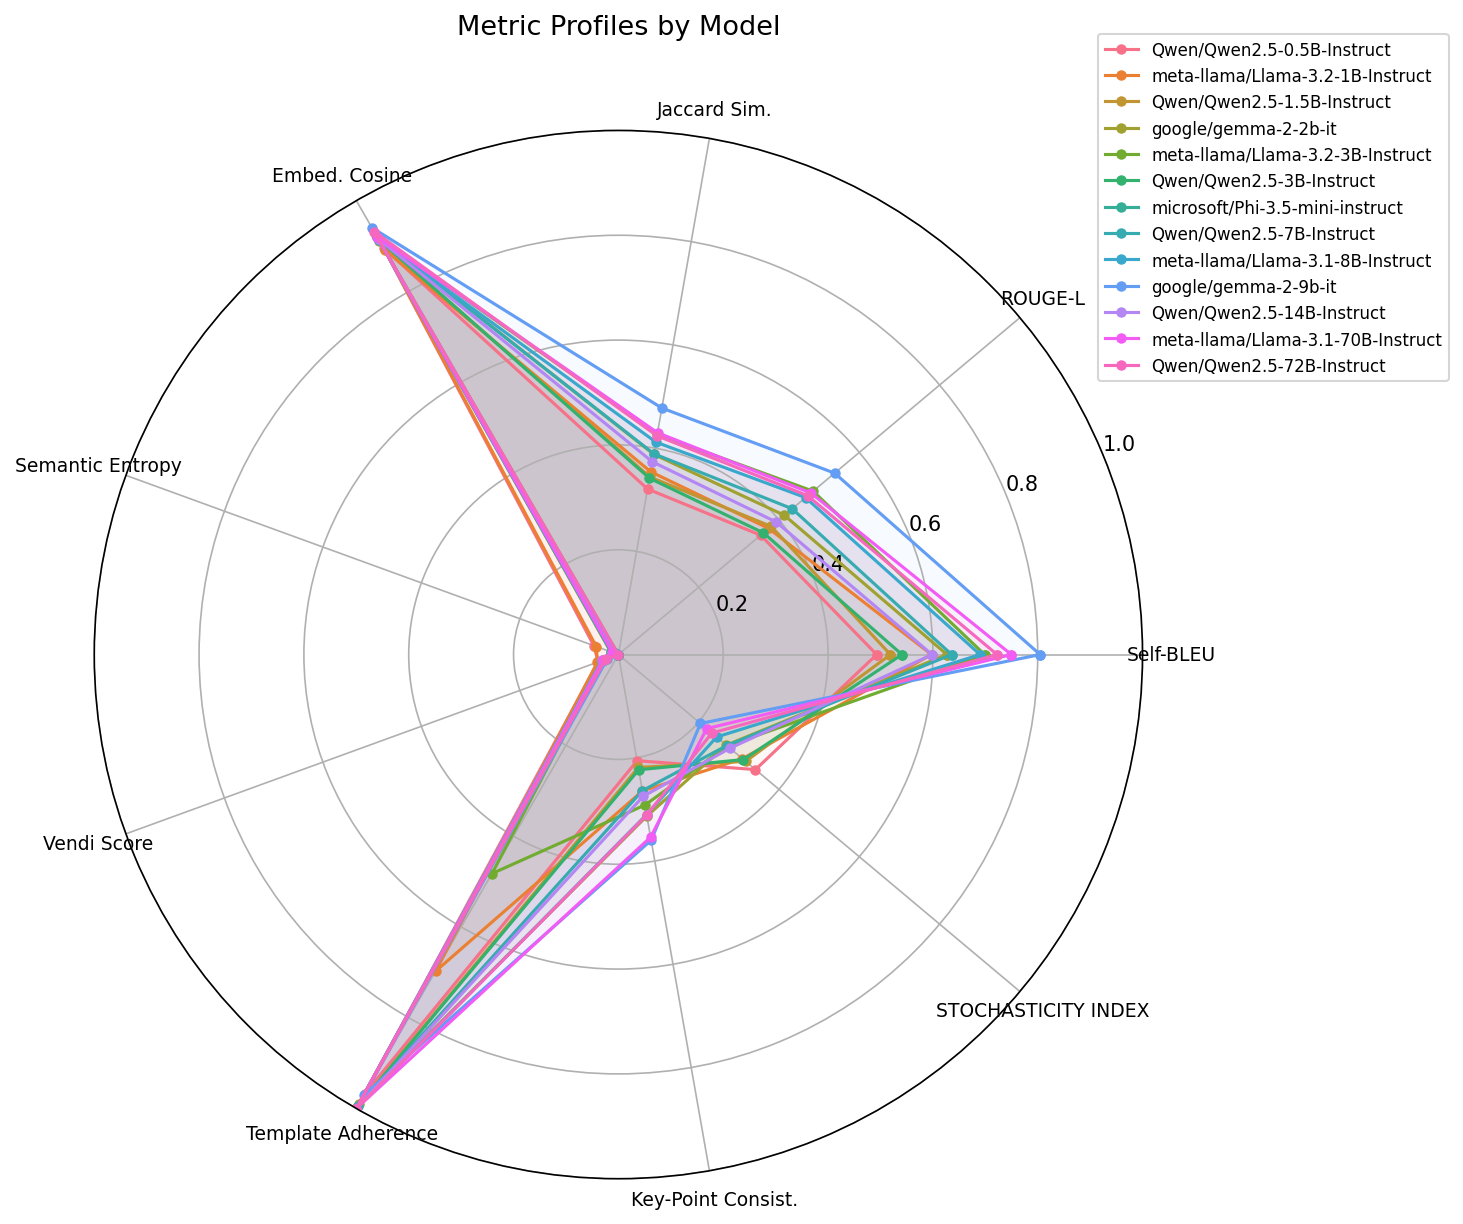
\includegraphics[width=\linewidth]{figures/radar_chart.png}
\caption{Radar chart of metric profiles across all models. Larger models (darker lines) cluster tightly toward the centre-right (high similarity, low entropy), while smaller models (lighter lines) extend further on diversity axes.}
\label{fig:radar}
\end{figure}

% ============================================================================
% 5. DISCUSSION
% ============================================================================
\section{Discussion}
\label{sec:discussion}

Our results paint a coherent picture: as language models grow larger, they become less stochastic across virtually every dimension of output variability we measured.
This section interprets these findings, identifies practical implications, and acknowledges limitations.

\subsection{Why Do Larger Models Exhibit Lower Stochasticity?}

We propose three complementary explanations for the observed scaling--stochasticity relationship.

\textbf{Sharper probability distributions.}
Larger models, having been trained on more data with more parameters, develop sharper conditional probability distributions over the next token.
When the probability mass is concentrated on fewer tokens at each generation step, the sampling process has less room for variation, even at the same temperature setting.
In effect, a temperature of 0.7 \emph{feels} more deterministic to a 72\,B model than to a 0.5\,B model because the underlying distribution is already more peaked.

\textbf{Better instruction following.}
Larger models are more adept at following the structured output template, which constrains the space of valid outputs.
A model that reliably produces a JSON object with five key points and three challenges has less room for variation than one that sometimes outputs free text, sometimes partial JSON, and sometimes valid JSON.

\textbf{Richer internal representations.}
Larger models have more capacity to build robust, stable representations of concepts.
When asked about ``AI in drug discovery,'' a 72\,B model likely activates a well-defined cluster of knowledge, leading to consistent outputs.
A 0.5\,B model, with sparser and noisier internal representations, is more susceptible to the randomness introduced by sampling.

\subsection{The Semantic Consistency Paradox}

One of our most striking findings is the contrast between high lexical stochasticity and near-zero semantic stochasticity.
Even the smallest models produce responses with embedding cosine similarities above 0.89, and semantic entropy values near zero.
This means that the \emph{information content} of responses is remarkably stable across runs---what varies is the \emph{expression} of that content.

This finding has important implications for evaluation methodology.
If we evaluate models using lexical metrics alone (as many benchmarks implicitly do through exact-match or F1 scoring), we may dramatically overestimate a model's inconsistency.
Semantic evaluation methods are essential for distinguishing genuine knowledge instability from harmless paraphrasing.

\subsection{Emergent Consistency: A New Perspective on Emergence}

Our tier-level analysis suggests that output consistency may itself be an emergent property.
The largest drop in stochasticity occurs between Tier~1 (below 3\,B) and Tier~2 (3--8\,B), coinciding with the parameter range where instruction-following capabilities are known to emerge.
This suggests a tantalising possibility: the same architectural changes that enable a model to reliably follow instructions also cause it to produce more consistent outputs.

If confirmed by future work, this would add ``output consistency'' to the list of emergent capabilities---capabilities that do not improve gradually with scale but instead appear relatively abruptly once a threshold is crossed.

\subsection{Practical Implications}

Our findings carry several practical implications for practitioners deploying LLMs.

\textbf{For reproducibility.}
Researchers evaluating small models should report results averaged over multiple runs, as single-run evaluations may be unrepresentative.
For models above 9\,B, single-run evaluations are more (though not perfectly) reliable.

\textbf{For safety-critical applications.}
In domains where consistency is paramount---clinical decision support, legal reasoning, financial analysis---our results favour larger models.
However, even the most consistent model in our study (Gemma-2-9b, SI~$= 0.205$) exhibits non-trivial variability, suggesting that deterministic generation settings or ensemble methods may be necessary for high-stakes applications.

\textbf{For model selection.}
Practitioners face a trade-off: smaller models are cheaper and faster but less consistent.
Our data provides quantitative guidance, showing approximately a 0.014-point reduction in SI per doubling of parameter count.

\textbf{For prompt engineering.}
Our prompt-level analysis shows that narrow, concrete prompts elicit more consistent responses than broad, open-ended ones.

\subsection{Limitations}

Several limitations constrain the generalisability of our findings.

\textbf{Single domain.}
All 20 prompts concern AI in healthcare.
While the within-domain variation provides breadth, we cannot confirm that the scaling--stochasticity relationship holds for fundamentally different domains (\eg, creative writing, mathematics, code generation).

\textbf{Fixed decoding parameters.}
We used a single temperature (0.7) and top-$p$ (0.9) setting.
The interaction between decoding parameters and model size is an important open question.

\textbf{One model excluded.}
Microsoft Phi-3.5-mini-instruct (3.8\,B) failed all 400 generation attempts due to a library incompatibility.
Its exclusion does not affect our conclusions, as Tier~2 retains three other models.

\textbf{Quantisation effects.}
Models above 65\,B were quantised to 4-bit precision.
While standard practice, this introduces a confound: we cannot fully separate the effect of model size from reduced precision.

\textbf{Limited frontier representation.}
Only two models represent the 70\,B+ tier.
A larger sample at this scale would strengthen the frontier analysis.

\subsection{Future Work}

This study opens several directions for future investigation.
Extending the analysis to multiple domains would test generalisability.
Varying decoding parameters systematically would reveal how model size interacts with sampling strategy.
Analysing individual token-level probability distributions could elucidate the mechanistic basis of the scaling effect.
Longitudinal studies tracking stochasticity across model versions could disentangle scale from training improvements.
Finally, fine-tuning experiments could test whether post-training alignment (RLHF, DPO) independently affects output consistency.

% ============================================================================
% 6. CONCLUSIONS
% ============================================================================
\section{Conclusions}
\label{sec:conclusion}

We have presented what is, to our knowledge, the first systematic multi-metric study of how LLM output stochasticity varies with model scale.
By evaluating 12 instruction-tuned models from three architectural families across a 144-fold range of parameter counts, we establish a clear and robust empirical finding: \textbf{larger language models are significantly less stochastic than smaller ones} (Spearman $\rho = -0.767$, $p = 0.004$).

This relationship is not a measurement artefact.
It holds across 11 of 13 evaluation metrics, spanning lexical, semantic, and structural dimensions.
It persists within each of the three model families tested.
And it is confirmed by a Kruskal--Wallis test showing statistically significant differences across four model-size tiers ($H = 137.78$, $p < 10^{-29}$).

At the same time, our analysis reveals an important nuance: the stochasticity that does exist is predominantly \emph{surface-level}.
Even the most variable models produce semantically consistent responses (embedding cosine similarity $> 0.89$), varying in phrasing and structure rather than in meaning.

These results have practical implications for reproducibility (multi-run evaluation is essential for small models), model selection (the consistency cost of choosing a smaller model is now quantifiable), and safety-critical deployment (even frontier models require additional controls for high-stakes use).
They also contribute to the theoretical understanding of emergence, suggesting that output consistency may itself be an emergent property that crystallises in the 3--8\,B parameter range.

As LLMs increasingly serve as the backbone of real-world applications, understanding not just \emph{what} they say but \emph{how reliably} they say it becomes essential.
Our work provides a methodological framework and empirical baseline for this investigation.

% ============================================================================
% BACK MATTER
% ============================================================================
\section*{Data Availability}
The complete dataset of 4\,800 model responses, evaluation metrics, and analysis code is available at: \url{https://github.com/khashayarghamati/Is-LL-MDeterministic-}

\section*{Acknowledgements}
This research was supported by computational resources provided by the University of Hertfordshire GPU cluster.

% ============================================================================
% REFERENCES
% ============================================================================
\bibliographystyle{plainnat}
\bibliography{references}

\end{document}
